\section{Ziel}
    Ziel dieses Versuches ist es Halbleiter-Nanokristall-Quantenpunkte auf ihre elektronischen Eigenschaften zu untersuchen.
    Dazu wird ihre Emissionsenergie bestimmt und die Abhängigkeit ihrer Photolumineszenzspektren von der Polarisation, Wellenlänge und Leistung des Lichtes betrachet.
    
\section{Theoretische Grundlagen}
  \subsection{Herstellung}
    Die Synthese der Nanokristalle kann in eine Nuklidbildung und das anschließende Wachstum der Nuklide unterteilt werden.

    Im ersten Schritt wird ein Lösungsmittel, welches ebenfalls als Stabilisator dient, auf ca. 330°C erhitzt und darin Cadmiumdimethyl und Hexadecylamin bei einer Temperatur von etwa 20°C injiziert. Dabei kommt es zur Bildung von $(Cd^{2+}, Se^{2-})_3$ Monomeren, welche sich zu Kristallisationskeimen entwickeln.
    Diese Reaktion hat eine Senkung der Temperatur zur Folge, welche den Prozess der Nuklidbildung beendet.
    Bei eine Temperatur von ca. 290°C werden die Keime auf den geschwünschten Durchmesser wachsen gelassen.
    Bei hoher Temperatur und damit ebenfalls hoher Monomerkonzentration wird von kinetischem Wachstum gesprochen, wohingeben bei kleinerer Temperatur bzw. Monomerkonzentration das thermodynamische Wachstum dominiert, welches versucht die Oberflächenenergie zu minimieren.
    Durch Abkühlen kann die Herstellung des Kerns der Nanokristalle abgeschlossen werden.

    Anschließend wird Zinksulfid in die Lösung gegeben, sodass der $CdSe$-Kern durch die $ZnS$-Schale isoliert wird.
    Die enstehenden Nanokristalle sind nahezu kugelförmig \textit{(siehe \ref{fig:NK} links)} und können durch die Länge der Wachstumsphase in ihrer Größe varriert werden.
    Typischerweise befinden sich Nanokristalle in der Größenordnung von $\sim 1-100\,\text{nm}$.
    \begin{figure}[h]
      \centering
      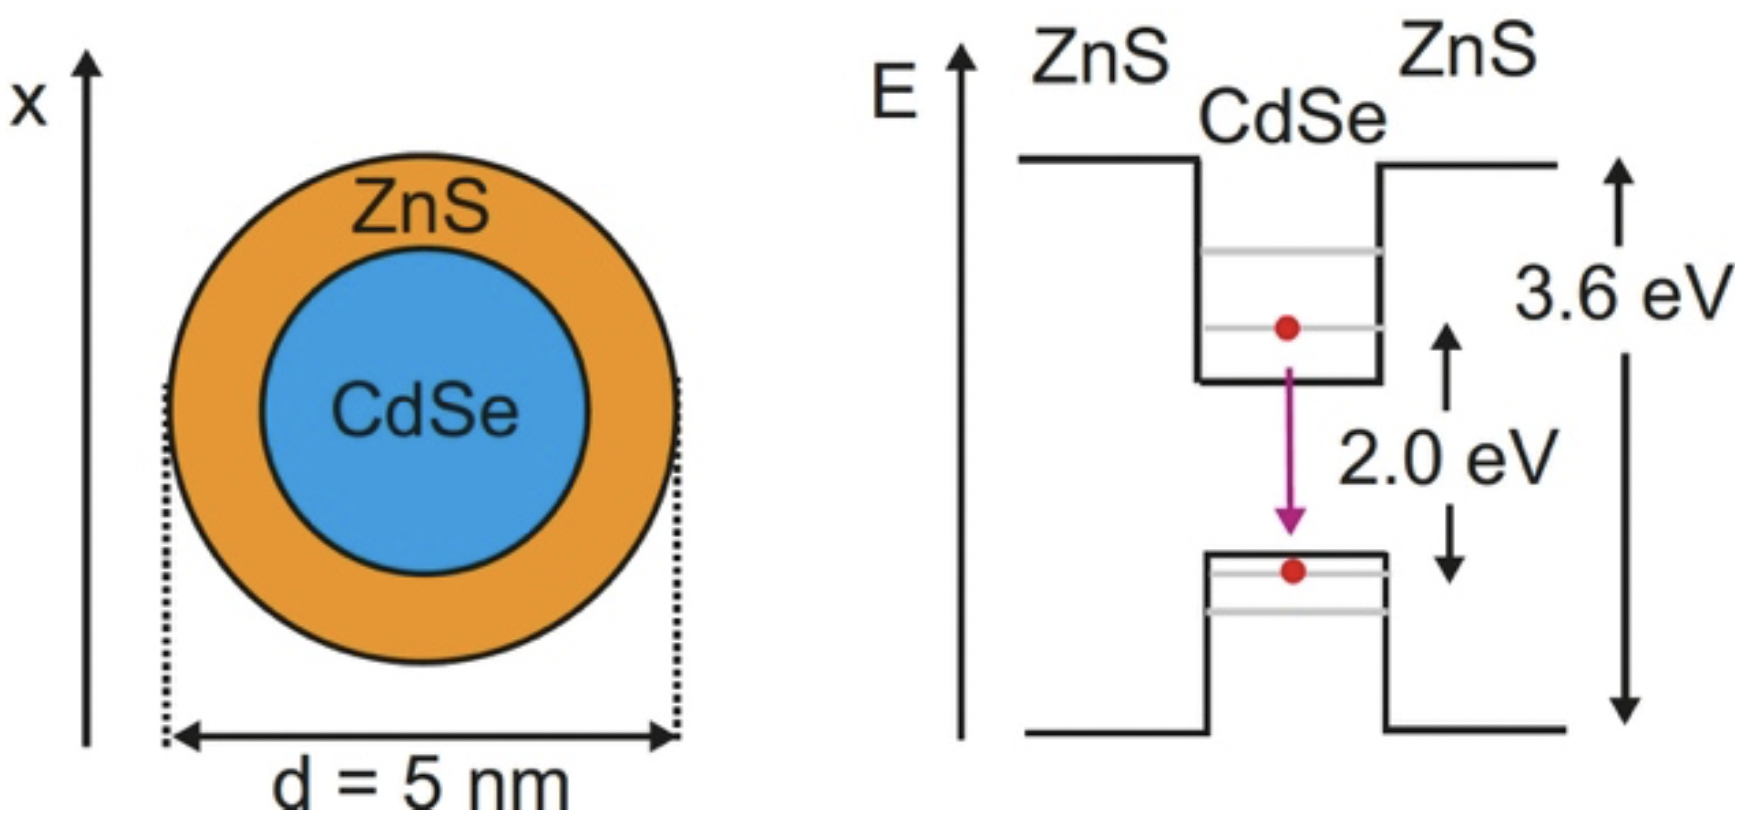
\includegraphics[width = 0.6\textwidth]{pictures/Nanokristalle.png}
      \caption{Schematische Darstellung des Aufbaus und der Ausmaße eines $CdSe/ZnS$ Quantenpunktes und seiner Energiestruktur. Entnommen aus \cite{tu_dortmund_versuchsanleitung_2021-6}}
      \label{fig:NK}
    \end{figure}

  \subsection{Elektronische Eigenschaften}
    Da die Bandlücke des $CdSe$-Kerns kleiner ist als die der $ZnS$-Schale erfährt die Wellenfunktion dadurch eine Einschränkung in allen drei Raumrichtungen durch die so entstehende Potentialbarriere. Diese ist in Abbildung \ref{fig:NK} zu sehen.
    Aufgrund der kleinen Größe der Nanokristalle führt das zu einer Quantisierung der Energiezustände, wie es bei einzelnen Atomen der Fall ist.
    \subsubsection{Photolumineszenz}
      Wird Licht mit einer genügend hohen Energie eingestrahlt, so kann ein Elektron in der $ZnS$ Barriere aus dem Valenzband in das Leitungsband angeregt werden. Es entsteht ein Elektron-Loch-Paar, auch Exziton genannt. Dieses kann von dem Quantenpunkt eingefangen und lokalisiert werden. Dort relaxieren das Elektron und das Loch jeweils über nicht-strahlende Streuprozesse an Phononen und Defekten zu den Kanten des Leitungs bzw. Valenzbands, wo sie unter Emission eines Photons rekombinieren.
      Dieser Vorgang ist in Abbildung \ref{fig:Prozess} dargestellt.
      \begin{figure}[h]
        \centering
        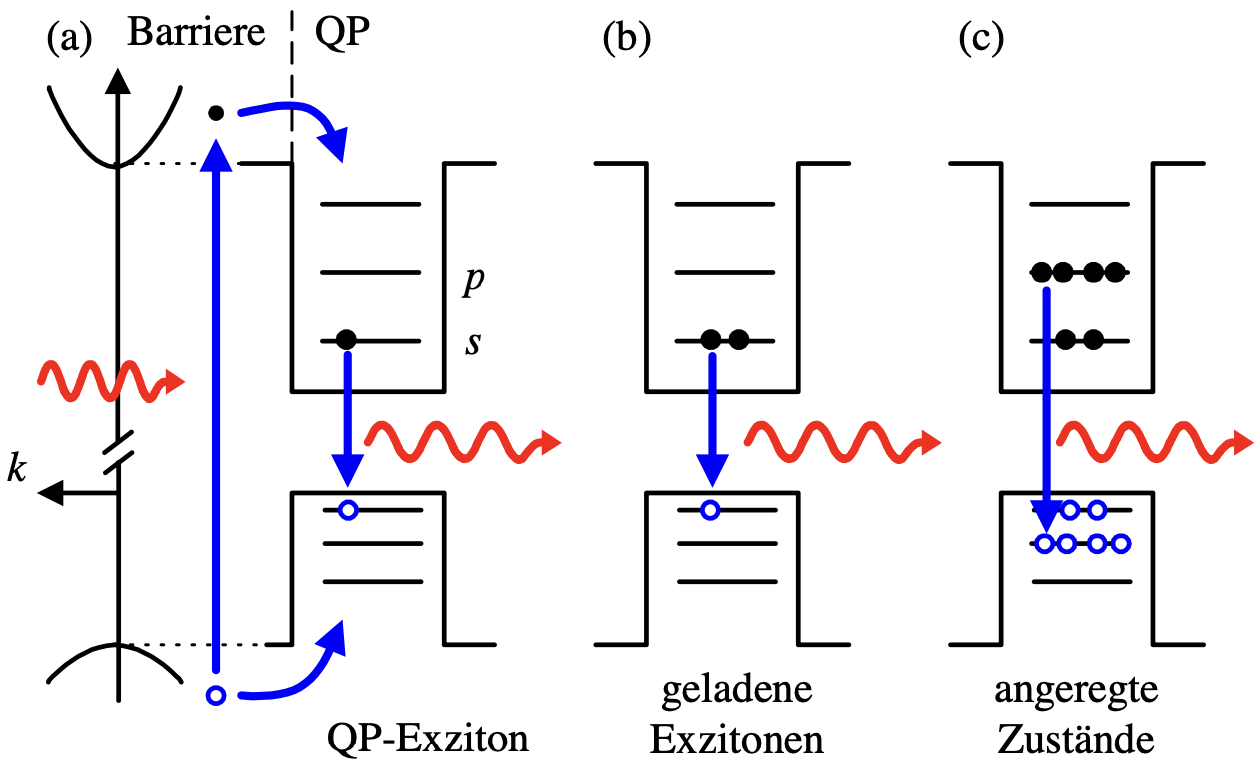
\includegraphics[width = 0.6\textwidth]{pictures/Prozess.png}
        \caption{\textit{a)} Photolumineszenz durch Einfangen von Exzitonen durch den Quantenpunkt. \textit{b)} Geladene Exzitonen durch Anwesenheit einer weiteren Ladung an der Bandlücke. \textit{c)} Rekombination aus angeregten Zuständen durch das Einfangen mehrerer Exzitonen bei hohen Anregungsdichten. Entnommen aus \cite{tu_dortmund_versuchsanleitung_2021-6}}
        \label{fig:Prozess}
      \end{figure}
      Die Rekombinationsenergie, also die Energie des ausgesendeten Photons
      \begin{equation}
          E_R = E_g + \frac{\pi^2\hbar^2}{ 2  a^2} \left(\frac{1}{m_e^*} + \frac{1}{m_h^*}\right) -\frac{\mu e^4}{32\pi^2\varepsilon_0^2 \varepsilon_r^2 \hbar^2}
          - 1.786\cdot \frac{e^2}{4\pi\varepsilon_r\varepsilon_0 a}.
      \end{equation}
      berechnet sich aus der Bandlücke $E_g$ über welche das Elektron-Loch-Paar relaxiert, also der quantisierten Zustände. Der zweite Summand beschreibt jeweils die Energie des Elektrons bzw. des Lochs und der dritte Summand die Exzitonenbindungsenergie, welche durch die Coulomb-Wechselwirkung zwischen Elektron und Loch gegeben ist. Der letzte Term berücksichtigt räumliche Einschränkung, die sowohl das Elektron als auch das Loch erfährt.
      $m_{e\,\text{bzw.}\,h}^*$ ist dabei die effektive Masse der rekombinierenden Teilchen, $\epsilon_0$ und $\epsilon_r$ die Permeabilitäten, $\mu=\frac{m_e^*\cdot m_h^*}{m_e^* + m_h^*}$ die sogenante reduzierte Masse und $a$ die Größe der Nanokristalle.

      Somit lässt sich die Farbe des ausgestrahlten Lichtes über die Größe der Nanokristalle $a$, wie in Abbildung \ref{fig:Farbe} zu erkennen einstellen.
      \begin{figure}[h]
        \begin{subfigure}{0.48\textwidth}
          \centering
          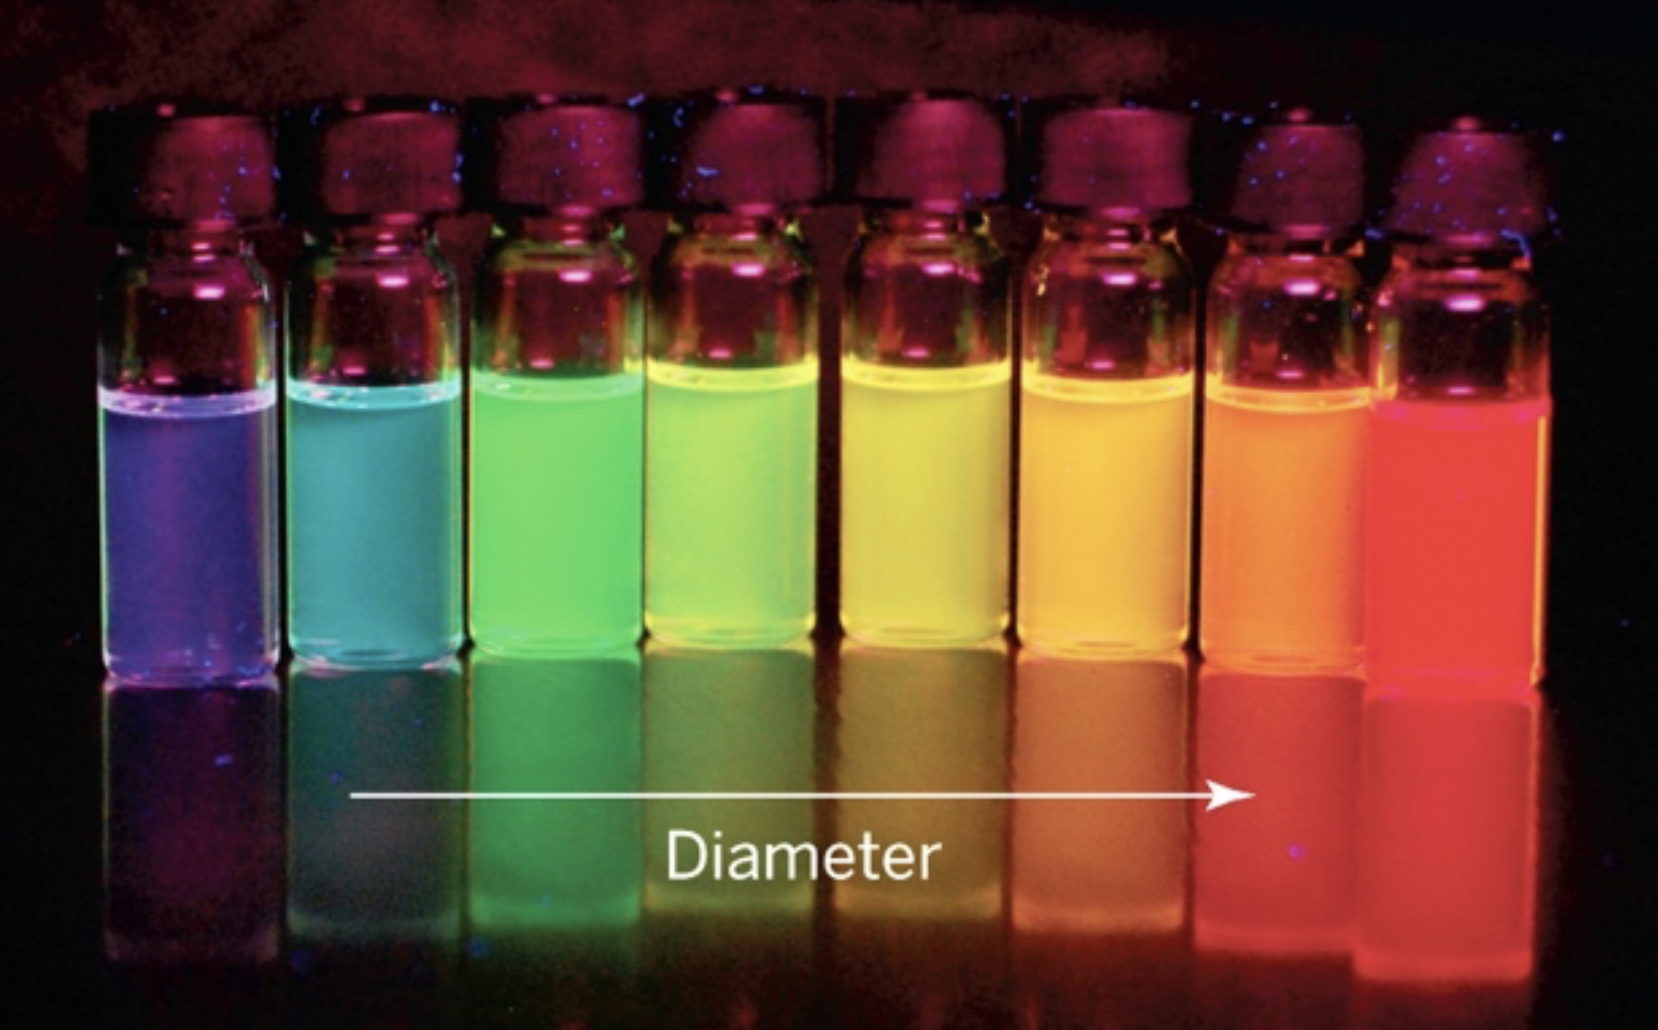
\includegraphics[height=4.5cm]{pictures/Farbe.png}
        \end{subfigure}
        \hfill
        \begin{subfigure}{0.48\textwidth}
          \centering
          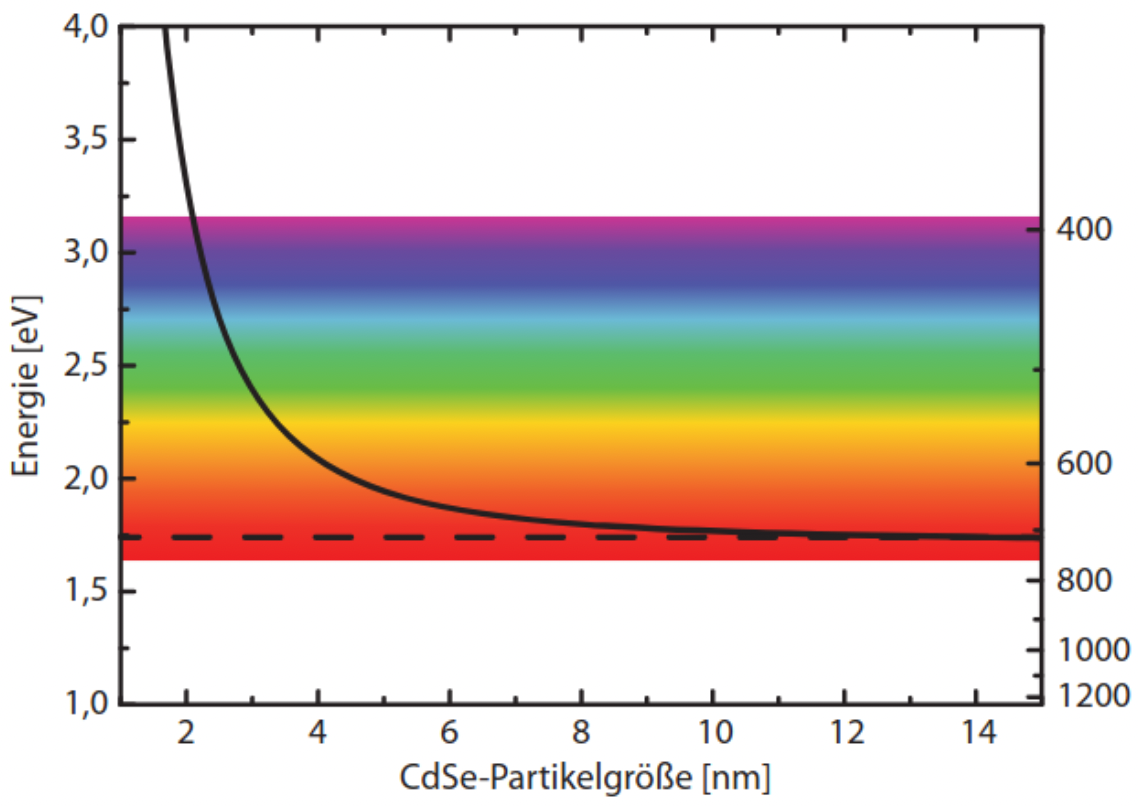
\includegraphics[height=4.5cm]{pictures/Farbe2.png}
        \end{subfigure}
        \caption{Photolumineszenz von verschieden großen $CdSe$ Nanokristallen. \textit{(links)} Abhängigkeit der Wellenlänge bzw. Energie von der Größe der Quantenpunkte. \textit{(rechts)} Entnommen aus \cite{tu_dortmund_versuchsanleitung_2021-6}}
        \label{fig:Farbe}
      \end{figure}
      Befinden sich bereits Elektronen im Leitungsband und/oder Löcher im Valenzband, so kann es zu sogenannten geladenen Exzitonen kommen. Dabei entstehen kleine Verschiebungen in der Energie im Vergleich zum regulären Exziton.
      Falls weitere Exzitonen vom Quantenpunkt eingefangen werden, so enstehen z.B. Biexzitonen im Falle von zwei Exzitonen kommen. Bei besonders hohen Anregungsdichten können so viele Exzitonen in den Quantenpunkt geraten, dass eine Rekombination nicht mehr nur aus dem Grundzustand, sondern auch aus den angeregten Zuständen beobachtet werden kann, was zu einer noch größeren Abweichung in der Rekombinationsenergie führt. Diese Prozesse sind ebenfalls in Abbildung \ref{fig:Prozess} graphisch dargestellt.